\section{The Mixing Configuration Problem}
\label{sec:config-choices}

We present the first component of \olmix: a comprehensive empirical study of the configuration space of mixing methods. We begin by formalizing the data mixing problem and describing the offline mixing schema (\S\ref{sec:background}). Then, we enumerate the key design choices that must be made to configure an offline mixing method (\S\ref{sec:design_choices}).
Our main contribution is an empirical study of these design choices in \S\ref{sec:study}. 
These findings inform \base (\S\ref{sec:base_method}), the mixing method we used throughout Olmo 3 development.


\subsection{Background}\label{sec:background}

\subsubsection{The Data Mixing Problem}\label{sec:setup_1}

Our goal is to determine ratios over training data domains that result in strong downstream performance.


\textbf{Domain set and mixes.} Let $\D = \{D_1, D_2, \dots, D_m \}$ be a set of $m$ domains, where each domain $D_i$ has a training dataset of size $N_i$ tokens. A domain is a group of data, ranging from coarse-grained \textbf{sources} (defined by data provenance) to fine-grained \textbf{topics} (semantically coherent partitions of a source)~\citep{wettig2025organizewebconstructingdomains}.
We specify a data mixture via a probability vector $p \in \triangle^{m-1}$, such that training on $R$ total tokens uses a dataset with $p_i \cdot R$ tokens from $D_i$ for each domain $i$.




\textbf{Model and evaluation.} We train a target LM of $S$ parameters for $R$ tokens on $p$, denoted as $\LM(S, R, p)$.
We then evaluate this model on a suite of $n$ downstream tasks. 
We measure the performance $f_i(\LM(S, R, p))$ on each task $i$ in terms of bits-per-byte (BPB), the negative log likelihood of the correct answer normalized by answer length in UTF-8 bytes. \citet{heineman2025signalnoiseframeworkreducing} showed that BPB can be used for decision-making at small model scales and \citet{huang2024compression} showed that BPB sets correlate with downstream performance across capabilities and model families.


\textbf{Goal.} Given a domain set $\D$ and target model configuration of $S$ parameters and $R$ tokens, we aim to find a mixture $p^\star$ that minimizes the average BPB across all downstream tasks---that is, minimizing $\frac{1}{n} \sum_{i = 1}^n f_i(\LM(S, R, p))$.


\subsubsection{The Offline Mixing Schema}\label{sec:schema}

Many existing methods follow an offline mixing schema to propose a mix; these methods are also described as ``function fitting-based offline methods'' in~\citet{liu2025rethinkingdatamixturelarge}'s survey. We describe the three steps of this schema below and present them in Figure~\ref{fig:schema} as well. 

\textbf{Step 1: Swarm construction.} We sample the space of possible mixes by training a ``swarm'' of $K$ small proxy models of size $\Ssmall$ on $\Rsmall$ tokens, each with different mixture weights $p^1, p^2, \dots, p^K \in \triangle^{m-1}$ sampled from some distribution $\mathcal{P}$. We evaluate each proxy model on the downstream task suite to obtain $y_{ij} := f_i(\LM(\Ssmall, \Rsmall, p^j))$, the performance of the $j$th proxy model on the $i$th task, for all tasks over the entire swarm. Altogether, this creates a dataset $\{(p^j, \{y_{ij}\}_{i=1}^n)\}_{j=1}^K$ of mixture weights paired with their performance across all tasks.

  
\textbf{Step 2: Regression model.} We fit regression models using the above dataset to capture the relationship between the mixture weights and downstream performance. 
We learn a function $\hat{f} \in \F$, where $\hat{f}(p) \approx \frac{1}{n}\sum_{i = 1}^n f_i(\LM(\Ssmall, \Rsmall, p))$. This enables us to predict the average downstream BPB of a proxy model trained on any candidate mix $p$.

\textbf{Step 3: Mixture optimization.} We propose a mix by solving an optimization problem that uses the regression model $\hat{f}$ as a surrogate for true performance. This optimization problem takes the form $\underset{p \in \mathcal{S}}{\text{minimize}} \hat{f}(p)$, where $\mathcal{S} \subseteq \triangle^m$ denotes the feasible set, which may be the full probability simplex or a restricted subset.


\begin{figure}
    \centering
    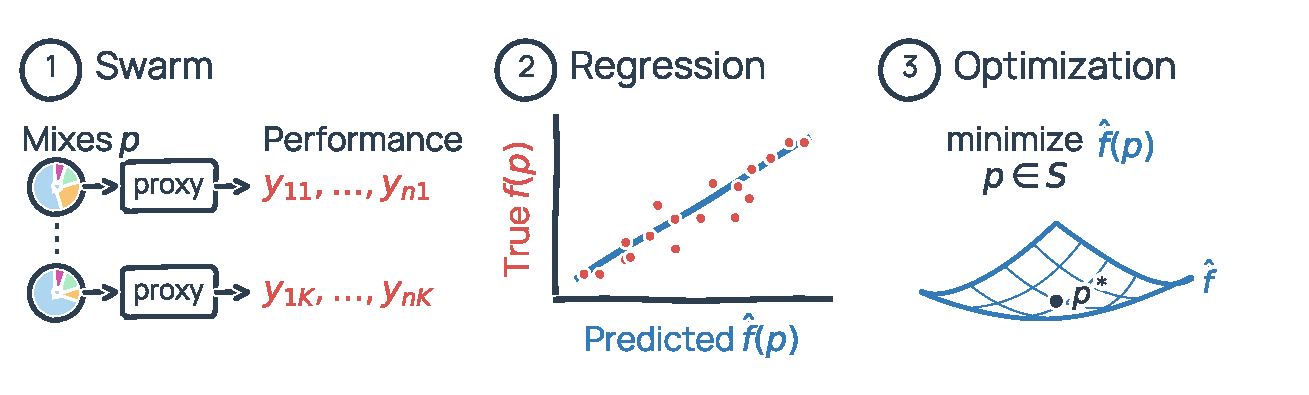
\includegraphics[width=\linewidth]{figs/fig_sro.pdf}
    \caption{The offline mixing schema used by many existing methods (\S\ref{sec:schema}). We study the design choices needed to configure the schema to develop a strong mixing method (\S\ref{sec:design_choices}-\S\ref{sec:study}).}
    \label{fig:schema}
\end{figure}

\subsection{\olmix Design Choices}\label{sec:design_choices}

Key design choices of the offline mixing schema are not explicitly identified in existing literature. We articulate these design choices as a configuration checklist of research questions (RQs) that practitioners must consider when developing their own mixing methods.

\begin{tcolorbox}[colback=ai2offwhite,colframe=black,boxrule=0.5pt,arc=3pt,left=6pt,right=6pt,top=6pt,bottom=6pt]
\textbf{Swarm construction:}
\begin{itemize}[itemsep=0.00pt,topsep=0pt,leftmargin=30pt]
    \item[\emph{RQ1}] What is the smallest proxy model size (the number of parameters, $\Ssmall$) such that decision-making generalizes to larger target models?
    \item[\emph{RQ2}] How many proxy runs $K$ do we need to learn a good mix on $m$ domains?
    \item[\emph{RQ3}] How should we specify the distribution $\mathcal{P}$ to sample the mixes for the proxy runs?
\end{itemize}

\textbf{Regression model:}
\begin{itemize}[itemsep=0.00pt,topsep=0pt,leftmargin=30pt]
    \item[\emph{RQ4}] Is there an optimal family of regression models ($\mathcal{F}$) for predicting mix performance?
    \item[\emph{RQ5}] At what granularity should we fit the regression models in order to construct $\hat{f}(p)$?
\end{itemize}

\textbf{Mix optimization:}
\begin{itemize}[itemsep=0.00pt,topsep=0pt,leftmargin=30pt]
    \item[\emph{RQ6}] How do we mix under finite data constraints?
    \item[\emph{RQ7}] How do we solve the optimization problem?
\end{itemize}
\end{tcolorbox}



Table~\ref{tab:mixing_design_choices} shows how several existing methods address these design choices we identify. Shaded cells indicate design choices with reported justification while white cells represent those that lack sufficient explanation or exploration of alternatives. There are three takeaways:
\begin{itemize}[itemsep=0.00pt,topsep=0pt,leftmargin=12pt]
\item Many design choices lack guidance beyond the specific
instantiation; for instance, decisions on the swarm size
and distribution are rarely explained.
\item Even design choices that have justification lack consensus. For example, each existing method proposes a different regression model and reports strong regression fit to support it.
\item Critical aspects of LM development remain unaddressed, such as mixing under data constraints.
\end{itemize}

These gaps motivate a systematic investigation of the design choices within the offline mixing schema. 

\begin{table}[t]
    \centering
    \caption{Design choices across offline mixing methods. For each design choice and mixing method, we identify the method's configuration. We shade cells in pink if we found empirical justification for their configuration. In the final column, we present the configuration for \base.}
    \begin{footnotesize}
    \setlength{\tabcolsep}{3pt}
    \begin{tabular}
{L{2.0cm}C{1.9cm}C{1.9cm}C{1.9cm}C{1.9cm}C{1.9cm}C{1.9cm}C{1.9cm}}
        \toprule
        \sbf{Design Choice} & \sbf{RegMix}~\citep{liu2025regmixdatamixtureregression} & \sbf{DML}~\citep{ye2025datamixinglawsoptimizing} & \sbf{AutoScale}~\citep{kang2025autoscalescaleawaredatamixing} & \sbf{BiMix}~\citep{ge2025bimixbivariatedatamixing} & \sbf{ADMIRE-BayesOpt} \newline \citep{chen2025admirebayesoptaccelerateddatamixture} & \sbf{CLIMB}~\citep{diao2025climbclusteringbasediterativedata} & \sbf{\base (Algorithm~\ref{alg:base_method})} \\
        \midrule
        \rowcolor{midgrey}\multicolumn{8}{l}{\sbf{Swarm Construction}} \\
        \midrule
        Proxy model size & \cellcolor{ai2lightpink} 1M
 & \cellcolor{ai2lightpink} 70, 160, 305, 410M & Target & 280M & 1M, 60M & \cellcolor{ai2lightpink} 350M & \cellcolor{ai2lightpink} 30M \\
        Swarm size (vs $m$ domains) & 512 ($m=17$) & \cellcolor{ai2lightpink} 20 ($m=7$) & $2m+1$ & 4 & 101 ($m=17$) & \cellcolor{ai2lightpink} 112 ($m=21$) & \cellcolor{ai2lightpink} $3(m+1)$ \\
        Swarm distribution & Dirichlet with natural prior & Exponential grid & Exponential grid & Entropy-weighted & Dynamic & \cellcolor{ai2lightpink} Dirichlet with natural prior & \cellcolor{ai2lightpink} Dirichlet with natural prior (sparse for topics, dense for sources) \\
        \midrule
        \rowcolor{midgrey}\multicolumn{8}{l}{\sbf{Regression Model}} \\
        \midrule
        Regression model family & \cellcolor{ai2lightpink} LightGBM & \cellcolor{ai2lightpink} Log-Linear & \cellcolor{ai2lightpink} Power Law & \cellcolor{ai2lightpink} Power Law &  Gaussian Process & \cellcolor{ai2lightpink} LightGBM & \cellcolor{ai2lightpink} Log-Linear \\
        Regression granularity & Aggregated & Aggregated & Per-Task & Per-Task & Aggregated & Aggregated & \cellcolor{ai2lightpink} Per-Task \\
        \midrule
        \rowcolor{midgrey}\multicolumn{8}{l}{\sbf{Mixture Optimization}} \\
        \midrule
        Data repetition constraints & No & No & No & No & No & No & \cellcolor{ai2lightpink} Yes \\
        Optimization solver & Search & Search & Gradient Descent & Exact Solver & Search & Search & \cellcolor{ai2lightpink} Exact Solver with KL reg. \\
        \bottomrule
    \end{tabular}
    \end{footnotesize}
    \label{tab:mixing_design_choices}
\end{table}



\subsection{\olmix Study: Configuring a Mixing Method}\label{sec:study}


We conduct a comprehensive study of each design choice. 
We describe our experimental setup (\S~\ref{sec:study_setting}) and then investigate the design choices pertaining to each component of the offline mixing schema (\S~\ref{sec:swarm}-\ref{sec:optimization}).

\subsubsection{Experimental Setup}\label{sec:study_setting}

\textbf{Data.} We use DCLM~\citep{dclm} partitioned into 24 topic-based domains using WebOrganizer~\citep{wettig2025organizewebconstructingdomains}. See Table~\ref{tab:domain_sizes} for domain names and token counts. In Appendix~\ref{supp:study_details}, we also provide results for mixing over the final data sources of Table~\ref{tab:domain-updates-full}. 

\textbf{Model.} We train 1B parameter decoder-only transformer models using Olmo 2 architecture~\citep{olmo20242olmo2furious} to 100B tokens (5x Chinchilla). We use a batch size of 512, sequence length of 4096, and max learning rate of $0.0018$. See Appendix~\ref{supp:exp_details} for more details. 

\textbf{Evaluation.} We measure BPB (bits-per-byte) over gold responses on $52$ downstream tasks spanning math, code, and commonsense QA. 
For QA tasks, the gold continuation is the answer text; for math and code tasks it is a human-written response. 
We treat subtasks (e.g. MMLU or coding language subsets) as standalone tasks when taking an macro-average of BPB scores. See Table \ref{tab:eval_suite} for the entire list of tasks.

Unless otherwise specified, all experiments use DCLM topics as the set of domains and \base (\S~\ref{sec:base_method}, Algorithm~\ref{alg:base_method}) as the default configuration, varying only the component under study. Appendix~\ref{supp:study_details} provides full experiment details.

\subsubsection{Swarm Construction Study}\label{sec:swarm}

\textbf{RQ1: Proxy model size.} 
Proxy models must provide reliable signal that transfers to the target model's scale while ideally being small so that computational costs are low. Existing methods use sizes ranging from 1M to 400M parameters, making it unclear what size is sufficient.

We train many proxy–target model pairs, where each pair consists of a proxy model and a 1B target model trained on the same mixture ratios.
We compute the Spearman rank correlation between proxy and target model performance (average BPB) to quantify transfer; a high correlation indicates that rankings at the proxy scale predict rankings at the target scale, ensuring reliability of proxy swarm decisions. We consider proxy models of 1M, 15M, 30M, and 60M parameters with 5x Chinchilla multiplier.


Figure~\ref{fig:proxy_size} shows that proxy models with $\ge 15$M parameters achieve strong rank correlation ($\rho > 89$).
However, 1M models show significantly degraded correlation ($r = 73$), making them unreliable for guiding mixture decisions. This is in contrast to the recommendation of RegMix~\citep{liu2025regmixdatamixtureregression}\footnote{Investigating the public RegMix code, we found their 1M implementation is closer to 15M, which our results suggest is a good proxy size.}.
\textbf{For our setting, we use 30M parameter proxy models with 3B tokens (5x Chinchilla}), which achieves a Spearman correlation of 89.6 with 1B target models.


\begin{figure}
    \centering
    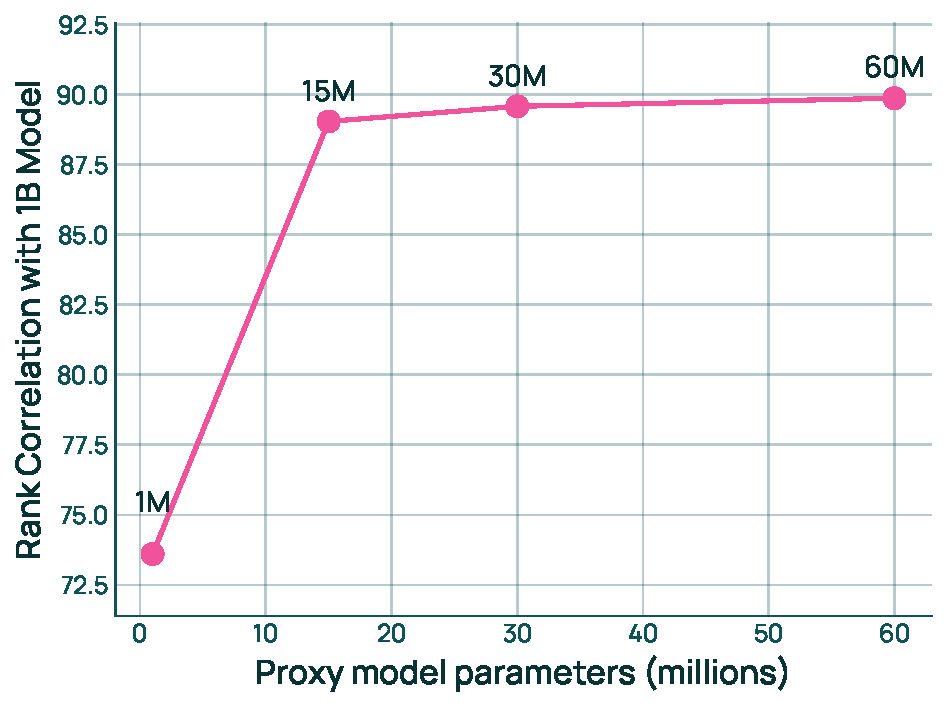
\includegraphics[width=0.5\linewidth]{figs/contribution_1/correlation_proxy_target.pdf}
    \caption{Correlation in performances between pairs of proxy models and 1B target models trained on the same mixture. Proxy models with over 15M parameters achieve strong rank correlation.}
    \label{fig:proxy_size}
\end{figure}






\textbf{RQ2: Swarm size in terms of number of domains.} 
The swarm size directly controls the cost-performance tradeoff: more proxy runs increase computational cost but improve mix quality. However, it is unclear what the tradeoff rate is when mixing over $m$ domains, since existing methods use fixed swarm sizes ranging from $20$ to over $500$, and few relate these choices to the number of domains $m$. 


We examine the sample complexity of the log-linear regression model, which we evaluate against other regression models in RQ4 and use in \base.  Specifically, given a set of $m$ domains, the sample complexity measures how many proxy runs $K$ are needed to produce a mix 
whose downstream BPB is within a certain margin of the best mix we've identified.
For a fixed number of domains $m$, we run a sweep over swarm sizes $K=c(m+1)$ for linear multiplier $c=1, 2, 3, 4, 5$ (since the minimum number of runs needed for a unique solution to log-linear regression is $m + 1$).
We perform this sweep for $m=6,12,18,24$ domains and $3$ seeds.
For each $m$, we define error as the difference between the BPB of a proposed mix and the best BPB achieved achieved by any mix found in the corresponding sweep for that $m$.
We used 30M proxy models for all runs here but verify that the proposed mixes from these different swarm sizes also exhibit the same trends at the 1B scale (Figure~\ref{fig:swarm_size_1B}).

Figure~\ref{fig:swarm_size} shows that sample complexity is linear in $m$: the error curves across $m$ collapse when plotted against the linear multiplier $c$.
This means that for any target error, there exists a fixed $c$ that achieves it, regardless of $m$.
Therefore, $\mathcal{O}(m)$ runs are sufficient for strong performance---a finding that contradicts prior assumptions of quadratic scaling~\citep{ye2025datamixinglawsoptimizing, ge2025bimixbivariatedatamixing} and provides practitioners with a concrete prescription for allocating compute. 
\textbf{We recommend using at least $K \ge 3(m+1)$ proxy runs with the log-linear regression model}, since $c = 3, 4, 5$ all have close to $0$ error. 

\begin{figure}
    \centering
    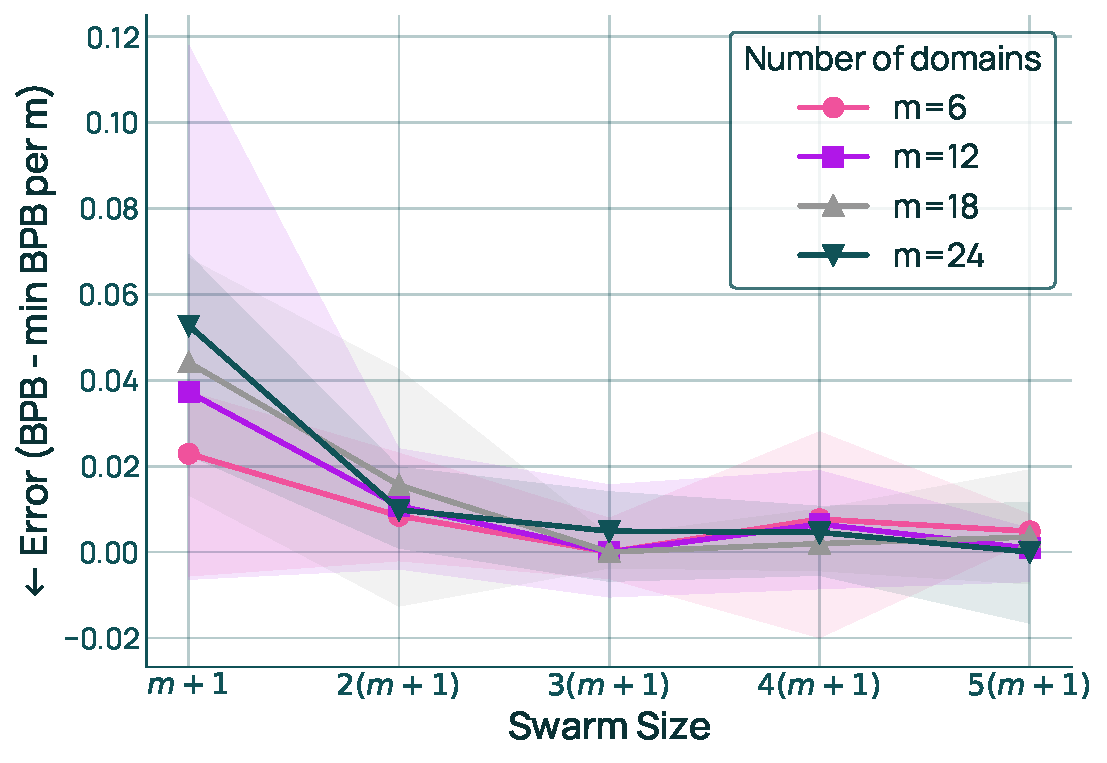
\includegraphics[width=0.5\linewidth]{figs/contribution_1/log_linear_sample_complexity_30M.pdf}
    \caption{Error vs. Swarm Size. Curves collapse across different $m$, indicating $\mathcal{O}(m)$ runs are needed. Results are averaged across 3 random seeds, and the intervals indicate min and max results.}
    \label{fig:swarm_size}
\end{figure}


\textbf{RQ3: Swarm distribution.} We study the distribution $\mathcal{P}$ from which swarm mixtures should be sampled. The distribution determines how effectively the swarm explores the mixture space. However, existing works rarely study the impact of the swarm distribution, with only CLIMB~\citep{diao2025climbclusteringbasediterativedata} comparing a Dirichlet versus a random uniform distribution. 


We investigate two aspects of the swarm distribution. To evaluate each aspect, we measure the average BPB of 1B target models trained on proposed mixes. As an intermediate metric, we also report the regression fit (Pearson correlation between predicted and true per-task BPB) on a held-out set of mixtures. 
\begin{itemize}
    \item \textit{Should each proxy run train on data from all domains (dense), or should some runs focus on subsets of domains (sparse)?} Sparse distributions enable discovering that certain domains should be excluded, while dense distributions ensure all domains are represented in all proxy runs. We generate sparse and dense swarms at the \textbf{topic level} (on DCLM topics) and \textbf{source level} (on the final sources from Table~\ref{tab:domain-updates-full}) to capture both fine and coarse-grained domains.
    
    \item \textit{Does centering the swarm around a promising mixture region improve results?} We test three Dirichlet priors: 1) the natural distribution (based on domain token counts), 2) a strong prior, and 3) a weak prior (see Appendix~\ref{supp:swarm_distribution} for exact constructions).
    
\end{itemize}


Figure~\ref{fig:swarm_distribution} shows that sparse swarms outperform dense at the topic level and vice versa at the source level—both for downstream BPB (left) and regression fit (right).
Neither is universally better; the choice depends on the domain set.
One hypothesis is that the best topic-level mixes exclude certain low-signal topics (e.g., adult content in DCLM), while the best source-level mixes utilize all sources. This aligns with how these domains were constructed: DCLM was partitioned into topics that are potentially uninformative, while sources are intentionally curated. \textbf{The choice of swarm distribution depends on the domain set; we recommend using sparse distributions for topic-level mixing and dense distributions for source-level mixing.}

Table~\ref{tab:dirichlet_priors} shows that centering on the natural distribution and the strong prior results in roughly similar downstream performance while using the weak prior significantly degrades performance. 
\textbf{We recommend that practitioners center the swarm around strong priors when available, but if prior knowledge is uncertain, the natural distribution remains a reasonable fallback.}


\begin{figure}
    \centering
    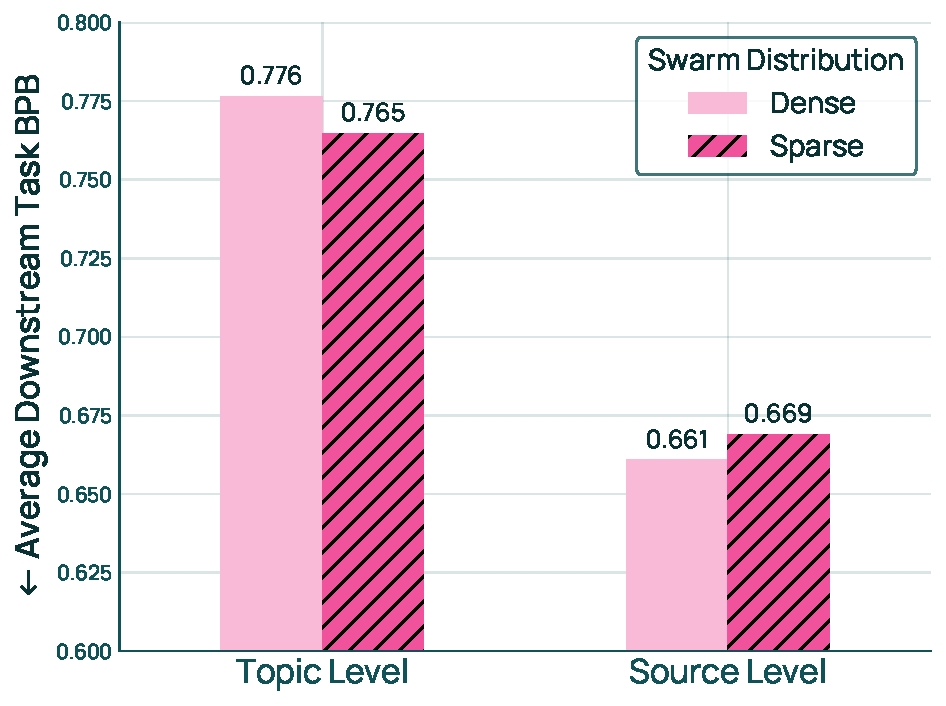
\includegraphics[width=0.47\linewidth]{figs/contribution_1/dense_vs_sparse_swarm_distribution.pdf}
    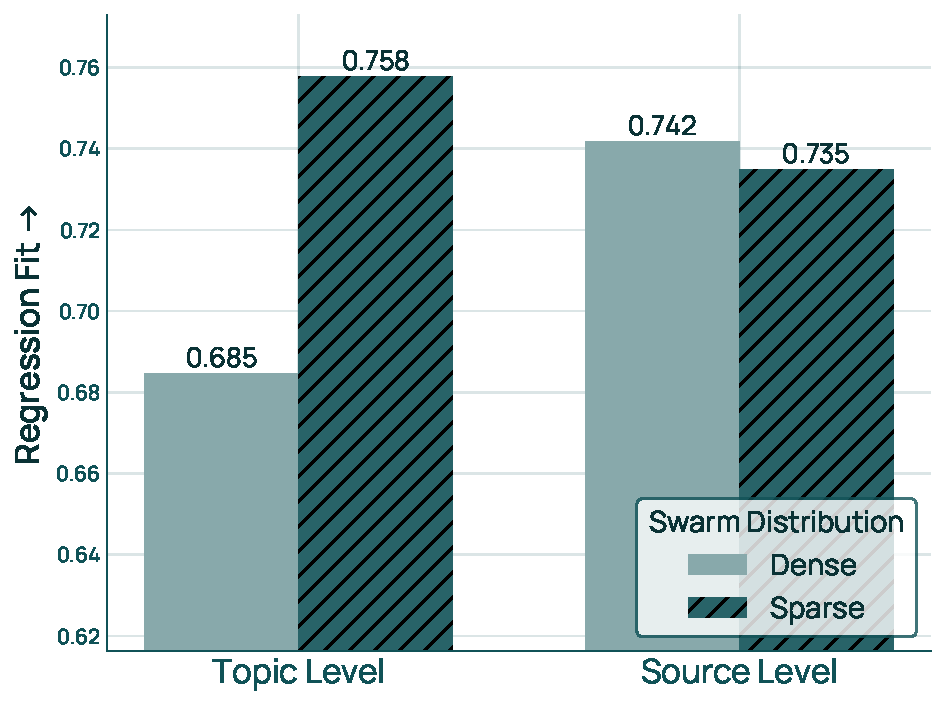
\includegraphics[width=0.5\linewidth]{figs/contribution_1/dense_vs_sparse_swarm_distribution_fit.pdf}
    \caption{Performance (left) and regression fit (right) of dense versus sparse swarms. While sparse swarms perform better at the topic level, dense swarms perform better at the source level, suggesting that behavior is data-dependent.}
    \label{fig:swarm_distribution}
\end{figure}

\begin{table}[t]
\centering
\caption{Natural and strong priors achieve similar downstream performance, but the weak prior does considerably worse, suggesting that this design choice is fairly robust and that the natural distribution is a reasonable configuration.}
\begin{tabular}{lcc}
\toprule
Dirichlet Prior & Avg Downstream Task BPB $\downarrow$ & Regression Fit $\uparrow$ \\
\midrule
Natural & 0.765 & 0.748 \\
Strong  & 0.763 & 0.835 \\
Weak    & 0.797 & 0.661 \\
\bottomrule
\end{tabular}
\label{tab:dirichlet_priors}
\end{table}


\subsubsection{Regression Model Study}\label{sec:regression}

\textbf{RQ4: Regression model family.}
The regression model is crucial: mixes are optimized directly using its predictions, meaning that regression fit directly controls the quality of the proposed mix.
However, each existing method proposes a different model and reports strong fit, making it unclear which to adopt.



We compare several regression model families derived from existing methods (see Appendix~\ref{supp:regression} for adaptations):
\begin{itemize}[itemsep=0.00pt,topsep=0pt,leftmargin=10pt]
    \item \textbf{Search}: selects the best mixture from the swarm.
    \item \textbf{LightGBM}~\citep{lightgbm}: a gradient boosting regression framework using decision trees. It has been used to learn the regression model in several mixing papers, including RegMix~\citep{liu2025regmixdatamixtureregression, wettig2025organizewebconstructingdomains, diao2025climbclusteringbasediterativedata}.
    \item \textbf{Gaussian Process}: based on~\cite{chen2025admirebayesoptaccelerateddatamixture}, we consider Gaussian Process regression with an RBF kernel scaled by a signal variance term and augmented with independent Gaussian observation noise.
    \item \textbf{BiMix}~\citep{ge2025bimixbivariatedatamixing}: we consider an adaptation of BiMix to our setting that has the following parametric form: $\hat{f}_i(p) = \sum_{j = 1}^m A_{ij} p_j^{-\alpha{ij}}$, where $A_{ij}, \alpha_{ij} \in \R^+$ for all $i, j$. 
    \item \textbf{AutoScale}~\citep{kang2025autoscalescaleawaredatamixing}: we consider an adaptation of Autoscale to our setting that has the following parametric form: $\hat{f}_i(p) = c_i + \sum_{j = 1}^m (R(A_{ij} + p_j))^{-\alpha_{ij}}$, where $c_i, \alpha_{ij} \in \R^+$, $A_{ij} \in [0, 1]$ and $R$ is the number of requested tokens for all $i, j$. 
    \item \textbf{Log-linear}: we consider an adaptation of Data Mixing Laws~\citep{ye2025datamixinglawsoptimizing} to our setting that has the following parametric form: $\hat{f}_i(p) = c_i + \exp(A_i^\top p_i)$, where $c_i \in \R^+$ and $A_i \in \R^m$ for all $i$. $m+1$ proxy models must be trained to obtain a unique solution.
\end{itemize}

First, we measure the regression fit, the Pearson correlation between predicted and true per-task BPB on held-out mixtures, across regression models and swarm sizes $K= 25, 50, 75, 100, 118$. We repeat this across 3 random seeds, subsampling each swarm from a pool of $118$ proxy runs (drawn from a larger swarm of $K=128$ with $10$ held-out mixes).


Figure~\ref{fig:regression_models} (left) shows that swarm size is a key confounding factor in regression fit: different models excel at different swarm sizes, potentially explaining the lack of consensus. For instance, BiMix~\citep{ge2025bimixbivariatedatamixing} performs the best for small swarms ($K=25$), while LightGBM~\citep{liu2025regmixdatamixtureregression} requires more than 118 proxy runs for sufficient fit. Notably, log-linear models~\citep{ye2025datamixinglawsoptimizing} achieve the best regression fit overall ($\rho=80$ at $K=118$) and outperforms other models consistently when  $K \ge 75$ (i.e. $K \ge 3(m+1)$).

Next, we examine the downstream performance of these regression models when $K=128$. Figure~\ref{fig:regression_models} (right) shows that the log-linear regression model's proposed mix achieves the best downstream performance. Combined with the strong regression fit, \textbf{we recommend using log-linear models}, given swarm size $K \ge 3(m+1)$, as recommended in RQ2.


Appendix~\ref{supp:regression} provides additional results at the source level (Figure~\ref{fig:regression_models_olmo3}) and how regression fit varies with swarm size and number of domains (Figure~\ref{fig:k_vs_m_dclm}).


\begin{figure}
    \centering
    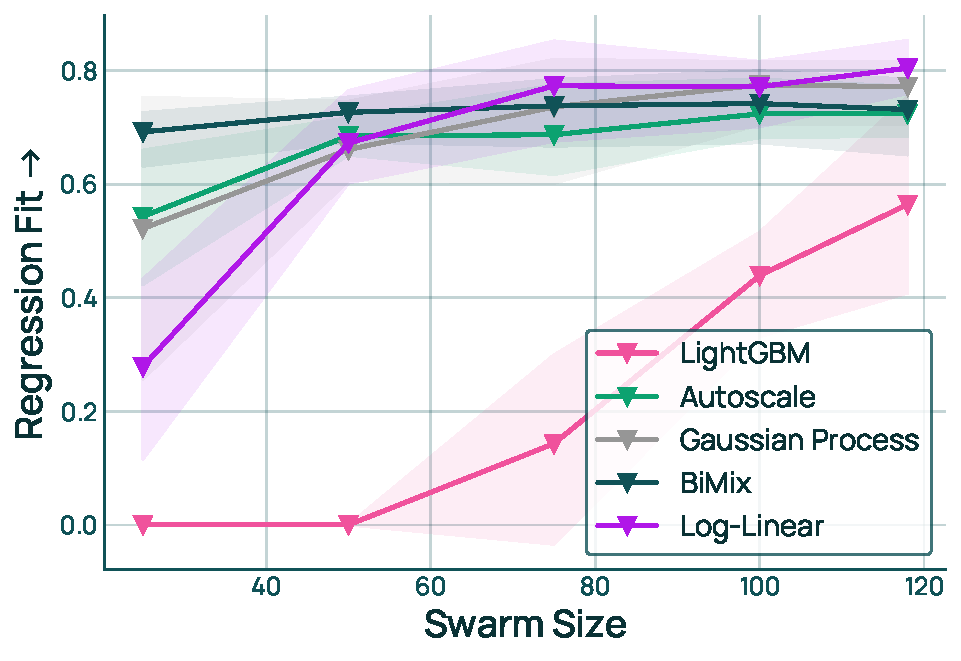
\includegraphics[width=0.48\linewidth]{figs/contribution_1/regression_models_24_domains_vs_k.pdf}
    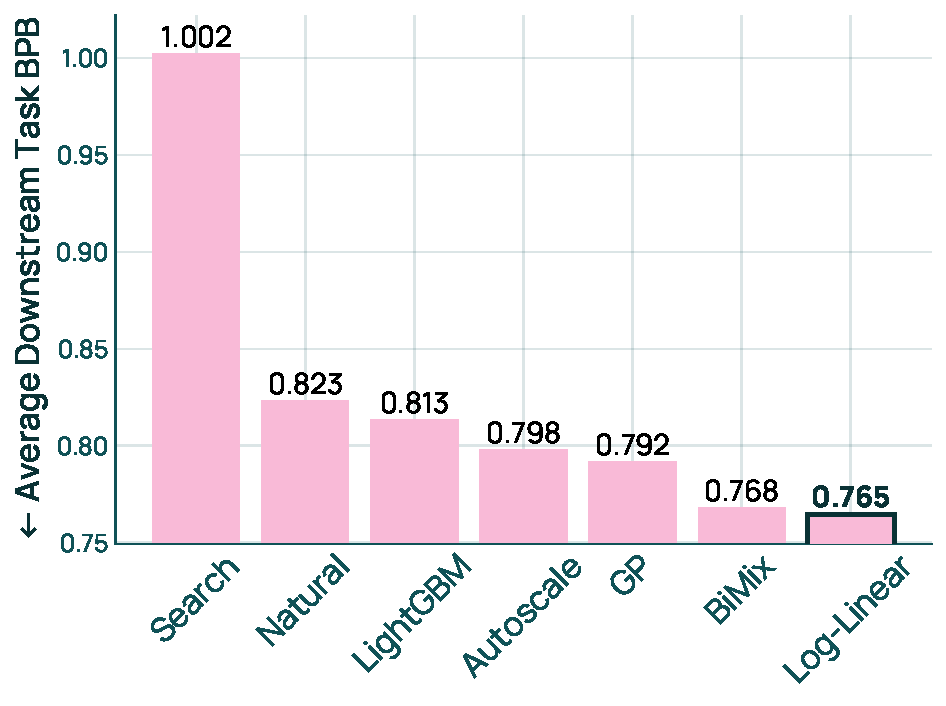
\includegraphics[width=0.48\linewidth]{figs/contribution_1/regression_models_performance.pdf}
    \caption{Left: Fit versus swarm size across regression models. Different models require different amounts of data, and the log-linear model achieves the best regression fit. Results are averaged across 3 random seeds, and the intervals indicate min and max results. Right: Downstream performance of regression models for $K=128$. The log-linear model achieves the best average downstream task BPB.}
    \label{fig:regression_models}
\end{figure}



\textbf{RQ5:Regression granularity.} We study the granularity at which to fit regression models in constructing $\hat{f}$: one model per task, one model per task family (e.g., math, code, and QA), or one model for the entire average BPB.
This involves a tradeoff between expressivity and noise. Per-task and per-family regression models can capture distinct relationships between mixtures and various capabilities, increasing expressivity of the overall function approximating average BPB, $\hat{f}$. 
However, they are fit to noisier individual measurements, while directly modeling average BPB may involve less noisy targets.



We compare three approaches. In the \textbf{per-task} approach, we fit individual functions $\hat{f}_i(p)$ using $\{(p^j, y_{ij})\}_{j=1}^K$ for each task $i \in [n]$, and then minimize $\frac{1}{n}\sum_{i = 1}^n \hat{f}_i(p)$. 
In the \textbf{per-family} approach, we group tasks into three families $F_1, F_2, F_3$: math, code, and QA. We fit one model $\bar{f}_i(p)$ to each family's average BPB using $\{(p^j, \frac{1}{|F_i|} \sum_{k \in F_i} y_{kj}) \}_{j = 1}^K$ for $i = 1, 2, 3$, and then minimize $\sum_{i = 1}^3 \frac{|F_i|}{n} \bar{f}_i(p)$.
In the \textbf{aggregated} approach, we fit a single function $\hat{f}_{\text{avg}}(p)$ directly to the average BPB across tasks using $\{(p^j, \frac{1}{n}\sum_{i = 1}^n y_{ij})\}_{j = 1}^K$ and minimize $\hat{f}_{\text{avg}}(p)$.  
We evaluate downstream performance (average BPB of 1B target models) and regression fit (Pearson correlation on held-out mixtures).



Table~\ref{tab:granularity} shows that per-task yields the best downstream performance and regression fit.
Regression fit degrades monotonically as granularity decreases, consistent with reduced expressivity.
While per-family has better regression fit than aggregated, their downstream performance is comparable; this is likely due to noise in transferring from proxy to target models since the performance on 30M models (Figure~\ref{fig:regression_granularity_30m}) exhibits trends that are consistent with the regression fit.
Nevertheless, per-task provides clear benefits on both metrics. \textbf{We recommend fitting separate regression functions per task.}


\begin{table}[t]
\centering
\caption{Performance and regression fit across regression granularities. As granularity of the regression target increases, the regression fit improves, and the downstream performance also trends towards improvement.}
\begin{tabular}{lcc}
\toprule
Method & Avg Downstream Task BPB $\downarrow$ & Regression Fit $\uparrow$ \\
\midrule
\rowcolor{ai2lightpink} Per-Task      & 0.765 & 0.983 \\
Per-Family    & 0.777 & 0.958 \\
Aggregated    & 0.774 & 0.866 \\
\bottomrule
\end{tabular}
\label{tab:granularity}
\end{table}



\subsubsection{Mix Optimization Study}\label{sec:optimization}

\textbf{RQ6: Data repetition constraints.}
In practice, LM training is often data-constrained: the target model’s requested training tokens $R$ exceed the available data. 
In this regime, some mixtures cause excessive sample repetition, degrading performance~\citep{muennighoff2025scalingdataconstrainedlanguagemodels}.
For example, a mixture that proposes 40\% code when code comprises only 5\% of available data would oversample code 8 times. Existing mixing methods assume compute-constrained settings with effectively infinite data and provide no way to control repetition. 



We consider repetition constraints of the form $p_j \le \frac{k N_j}{R}$ for all $j \in [m]$, where $k$ is a repetition factor that limits how many times any domain can be sampled given $R$ requested tokens and $N_j$ available tokens in domain $j$.
We study two questions around enforcing these constraints and their impact on proposed mixes.
\begin{itemize}
    \item \textit{How should repetition constraints be enforced while ensuring strong downstream performance?} 
    We consider two places where constraints can be enforced. First, we can constrain the swarm by ensuring that all swarm mixes satisfy the constraint---the regression models then learn what mixes are feasible. Second, we can constrain the optimization problem directly. This creates three approaches: 1) constrained swarm with unconstrained optimization, 2) unconstrained swarm with constrained optimization, and 3) constrained swarm with constrained optimization.     
    We test with $k=4$, verifying whether the proposed mixture satisfies the constraint and reporting downstream performance.
    
    \item \textit{How does the repetition factor affect the proposed mix?} Using the best-performing strategy, we vary $k \in \{2, 3, 4, 5, \infty \}$ and visualize how the proposed mix changes.

\end{itemize}


Table~\ref{tab:enforce_rep} shows that approach 2 (unconstrained swarm, constrained optimization) results in a proposed mix that satisfies the repetition constraints while maintaining performance. Approach 1 fails to satisfy the constraints, repeating samples from one domain 5 times and exceeding $k=4$. Approach 3 satisfies constraints but yields worse downstream performance than approach 2, likely because the constrained swarm provides less coverage of the mixture space. \textbf{We recommend enforcing repetition constraints in the mixture optimization step.}


\begin{table}[t]
\centering
\caption{Performance and repetition constraint satisfaction. Using a constrained swarm with unconstrained optimization does not satisfy a repetition constraint with $k=4$; the proposed mix repeats samples of a domain 5 times. Between approaches 2 and 3, the former approach achieves the best downstream performance.}
\begin{tabular}{lcc}
\toprule
Approach &
Satisfies rep.\ constraint? ($k=4$) &
Avg.\ Task BPB $\downarrow$ \\
\midrule
1) Constrained Swarm, Unconstrained Opt   & No (5)  & 0.774694 \\
\rowcolor{ai2lightpink}
2) Unconstrained Swarm, Constrained Opt  & Yes (4) & 0.764718 \\
3) Constrained Swarm, Constrained Opt    & Yes (4) & 0.785517 \\
\bottomrule
\end{tabular}
\label{tab:enforce_rep}
\end{table}


Figure~\ref{fig:vary_rep_top_7} shows how the proposed mix changes with varying $k$ when we add a repetition constraint to the optimization problem.. As the constraint relaxes from $2$ to $\infty$ (the infinite data setting), the mixture weights on high-utility domains, such as software development, monotonically increase. In contrast, domains such as literature smoothly decrease as $k$ increases, suggesting that their larger allocations under tight constraints primarily compensate for limited availability of higher utility domains. This demonstrates that repetition constraints significantly shape the proposed mix.


\begin{figure}
    \centering
    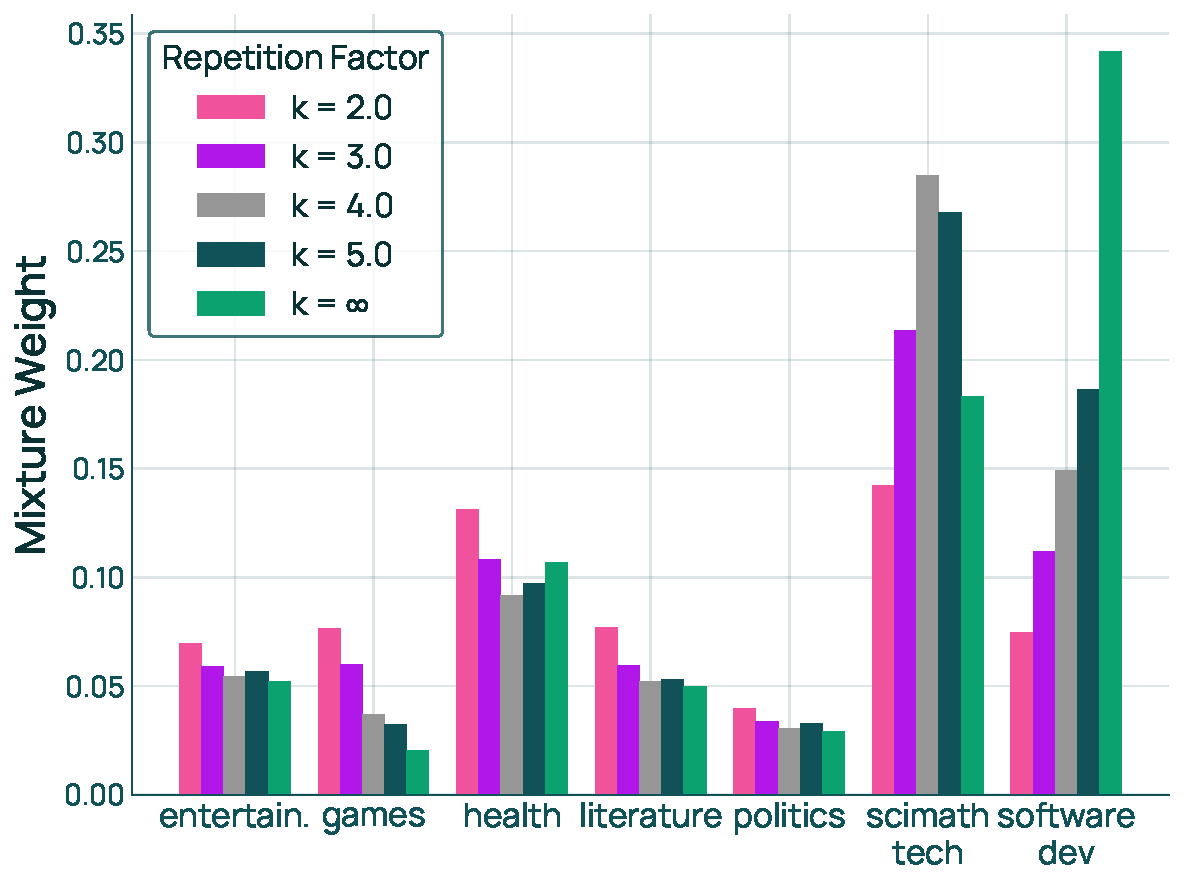
\includegraphics[width=0.5\linewidth]{figs/contribution_1/vary_repetition_factor_top_7.pdf}
    \caption{Proposed Mixture Weights versus Repetition Factor. Enforcing varying caps on repetition $k$ leads to significantly different proposed mixes. See Figure~\ref{fig:vary_repetition_factor} for mixture weights on the full set of domains.}
    \label{fig:vary_rep_top_7}
\end{figure}


\textbf{RQ7: Optimization solver.} We study how to solve for the mixture that minimizes the average predicted BPB $\hat{f}(p)$. Under log-linear regression, $\hat{f}(p)$ is convex, enabling exact solvers. However, since regression functions imperfectly predict performance (Figure~\ref{fig:regression_models} left), it is unclear whether exact optimization of the surrogate objective yields the mix with the best downstream performance or if incorporating some regularization may be better.


We consider three solving strategies. The \textbf{exact solver} uses CVXPY to compute the optimal mix. The \textbf{search}-based solver, used in RegMix~\citep{liu2025regmixdatamixtureregression}, samples candidate mixes from a Dirichlet distribution with a natural prior (i.e., a mix proportional to the domain sizes). The \textbf{exact solver with KL regularization} modifies the objective to $\text{minimize}_{p \in \triangle^{m - 1}} \hat{f}(p) + \lambda \kl(p || p_0)$, where $\lambda > 0$ controls the strength of regularization towards the natural distribution $p_0$; we consider $\lambda \in \{0.01, 0.05\}$. We measure the average BPB of 1B target models trained on the proposed mixes. We also examine the optimal objective value, the predicted average BPB at the 30M proxy model scale, as a sanity check that the exact solver should obtain the lowest predicted BPB.


Figure~\ref{fig:solvers} (left) shows that the exact solver with $\lambda=0.05$ achieves the best performance. In contrast, the right panel confirms that the exact solver obtains the lowest predicted BPB, while adding a KL penalty degrades it. Taken together, these results indicate that although the average predicted BPB is optimized most effectively by the exact solver, noise from regression fitting and proxy-to-target model transfer makes moderate regularization beneficial. The search baseline achieves poor performance, consistent with it being a heuristic. \textbf{We recommend using an exact solver with a KL regularization of 0.05 to solve the mixture optimization problem}. See Appendix~\ref{supp:solver}, Figure~\ref{fig:solvers_olmo3} for additional source-level results.

\begin{figure}
    \centering
    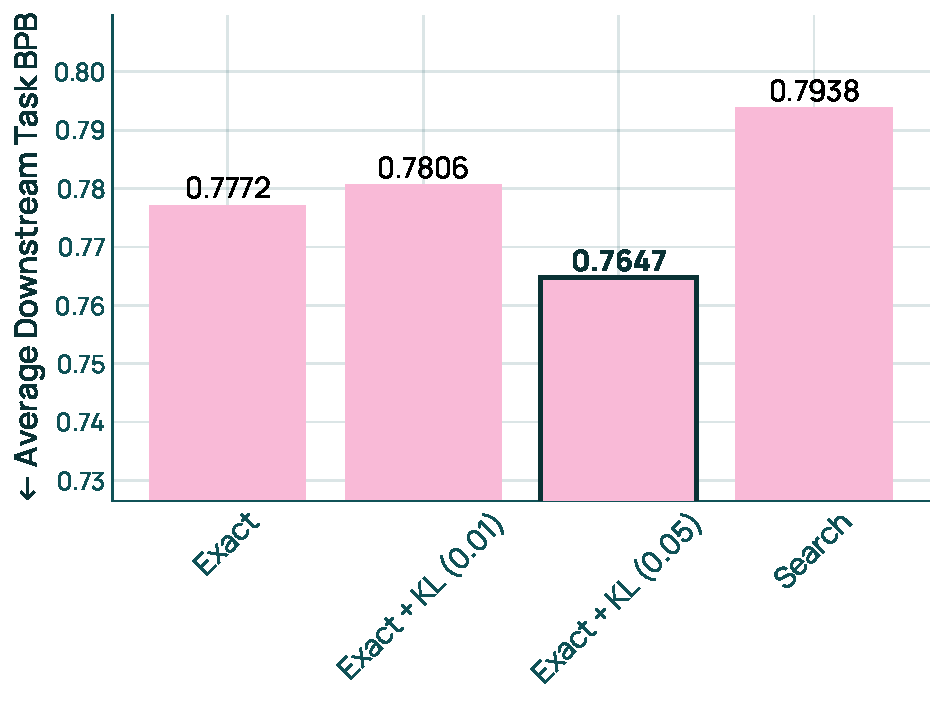
\includegraphics[width=0.48\linewidth]{figs/contribution_1/performance_solvers_dclm_6T.pdf}
    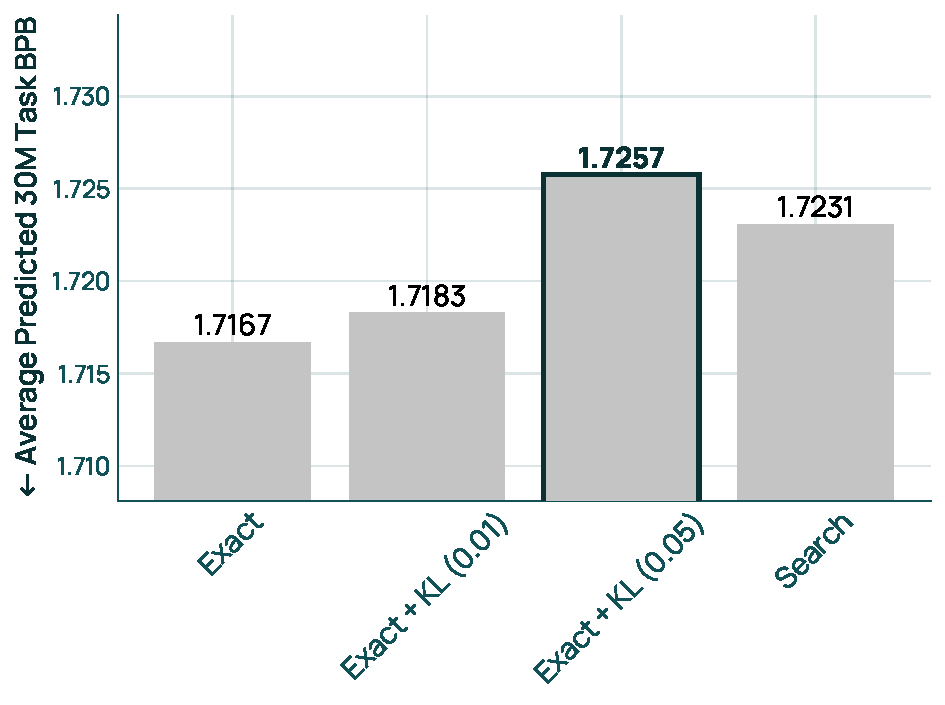
\includegraphics[width=0.5\linewidth]{figs/contribution_1/predicted_performance_solvers_dclm.pdf}
    \caption{Downstream performance (left) and 30M predicted performance (right) across optimization solvers. The predicted performances of various solvers confirms that the exact solver minimizes the predicted BPB, as expected, followed by KL penalties of $0.01$ and $0.05$. However, the exact solver does not obtain the best downstream performance, and instead some KL regularization helps.}
    \label{fig:solvers}
\end{figure}


\subsection{Configuring \base}\label{sec:base_method}


Our results in \S\ref{sec:study} let us define \base, a concrete configuration of the offline mixing schema that we use throughout Olmo 3 development. The rightmost column of Table~\ref{tab:mixing_design_choices} summarizes the full configuration, and Algorithm~\ref{alg:base_method} formalizes the procedure (\textcolor{olmoBlue}{blue} highlights steps informed by our findings).


\begin{center}
\begin{tikzpicture}
\node[inner sep=0pt] (alg) {
\begin{minipage}{0.9\textwidth}
\begin{algorithm}[H]
   \caption{\base}
   \label{alg:base_method}
\begin{algorithmic}[1]
   \STATE {\bfseries Input:} Domains $\D = \{D_1, \dots, D_m\}$ of sizes $\{N_1, \dots, N_m\}$, swarm size \textcolor{olmoBlue}{$K = \mathcal{O}(m)$}, repetition factor $k$, requested tokens $R$, KL penalty $\lambda$, natural distribution $p_0 \propto \{N_1, \dots, N_m \}$.  
    \STATE Sample mixes $p^1, \dots, p^K \in \triangle^{m-1}$ on $\D$.
    \STATE Train proxy models \textcolor{olmoBlue}{$\Ssmall\ge 15$M parameters} on these mixes, and evaluate on downstream tasks to get a dataset of mixes and performance, $\{(p^j, \{y_{ij}\}_{i = 1}^n \}_{j =1}^K$, where $y_{ij}:= f_i(\LM(\Ssmall, \Rsmall, p^j))$.
    \FOR{$i \in [n]$}
        \STATE Use $\{(p^j, y_{ij})\}_{j = 1}^K$ to fit the \textcolor{olmoBlue}{log-linear model} $\hat{f}_i(p) \texttt{=} c_i + \exp(A_i^\top p)$, where $c_i \in \R^+$ and $A_i \in \R^{m}$.
    \ENDFOR
    \STATE Solve the optimization problem to get $p^\star$:
    \begin{align*}
        &\text{minimize}_{p \in \triangle^{m-1}} \frac{1}{n} \sum_{i=1}^n \hat{f}_i(p) + \textcolor{olmoBlue}{\lambda \kl(p || p_0)} \qquad \text{subject to} \quad \textcolor{olmoBlue}{p_j \leq \frac{k N_j}{R} \; \forall j \in [m]} 
    \end{align*}
   \STATE \textbf{Return} $p^\star$.
\end{algorithmic}
\end{algorithm}
\end{minipage}
};

\draw [decorate,decoration={brace,amplitude=5pt}]
    ([yshift=-2.0cm,xshift=5pt]alg.north east) -- ([yshift=-3.6cm,xshift=5pt]alg.north east)
    node[midway,right=10pt,rotate=-90,anchor=south] {\footnotesize Swarm};

\draw [decorate,decoration={brace,amplitude=5pt}]
    ([yshift=-3.7cm,xshift=5pt]alg.north east) -- ([yshift=-4.9cm,xshift=5pt]alg.north east)
    node[midway,right=8pt,rotate=-90,anchor=south] {\footnotesize Regression};

\draw [decorate,decoration={brace,amplitude=5pt}]
    ([yshift=-5.0cm,xshift=5pt]alg.north east) -- ([yshift=-7.0cm,xshift=5pt]alg.north east)
    node[midway,right=8pt,rotate=-90,anchor=south] {\footnotesize Optimization};
\end{tikzpicture}
\end{center}
